%
% FIX THIS -- remove/change, just some examples of things
%


\chapter{Partially Observable Environments}

\section{Introduction}
%this is how an image should look
%\includegraphics{universe}
Until now, both the GTGR and GTGRD models have given the observer full knowledge of the adversary's state for the entirety of the game. In real-world environments, observers may not have perfect information regarding the states and actions of an adversary. 

To accommodate for scenarios with incomplete information for the adversary, we introduce a partially observable variant of the GTGR scenario. In partially observable scenarios, the rules of the game remain largely unchanged, except for addition of “shadow states." The observer can not discern the current state of the adversary, while the adversary occupies a shadow state. When the adversary enters an observable portion of the graph, the observer will become aware of the adversary's position once more.

\begin{figure}[h!]
\begin{center}

  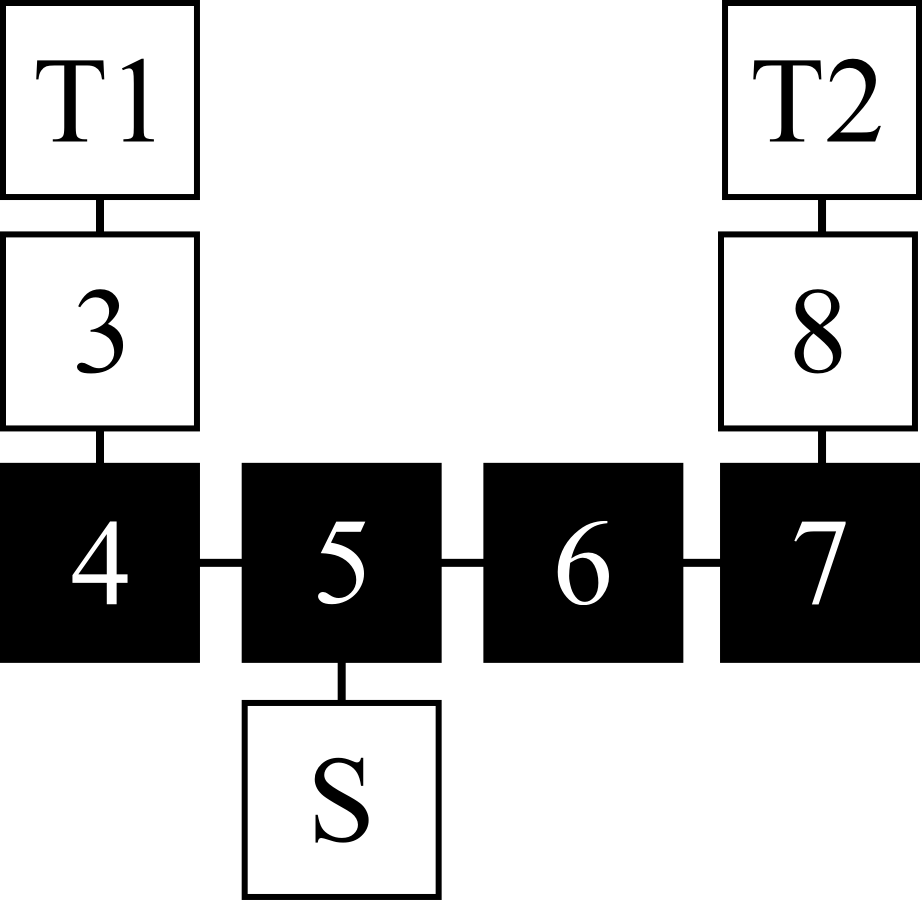
\includegraphics[scale=.15]{shadow1}
  \end{center}

  \caption{A partially observable graph.}
  \label{fig:shadow1}
\end{figure}

Figure~\ref{fig:shadow1} illustrates a partially observable environment. Visible states, in which the observer can see the adversary  white. Shadow states, in which the adversary is hidden from the observer, are black. The agent starts the game in state $S$. When the adversary moves to states $4$ ,$5$, $6$, or $7$, the observer is unable to determine their position until the adversary re-enters a visible portion of the graph.  
We will examine two solutions to the partially observable model, both of which involving linear programming. 

\section{The Whale Method}

The first method of solving partially observable environments, which we will call the "Whale Method," will utilize disjoint sets of shadow states. We call these sets of shadow states "shadow sets." We say that two shadow states belong to the same shadow set, if the adversary can travel between the two without entering an observable state.

\begin{figure}[h!]
\begin{center}

  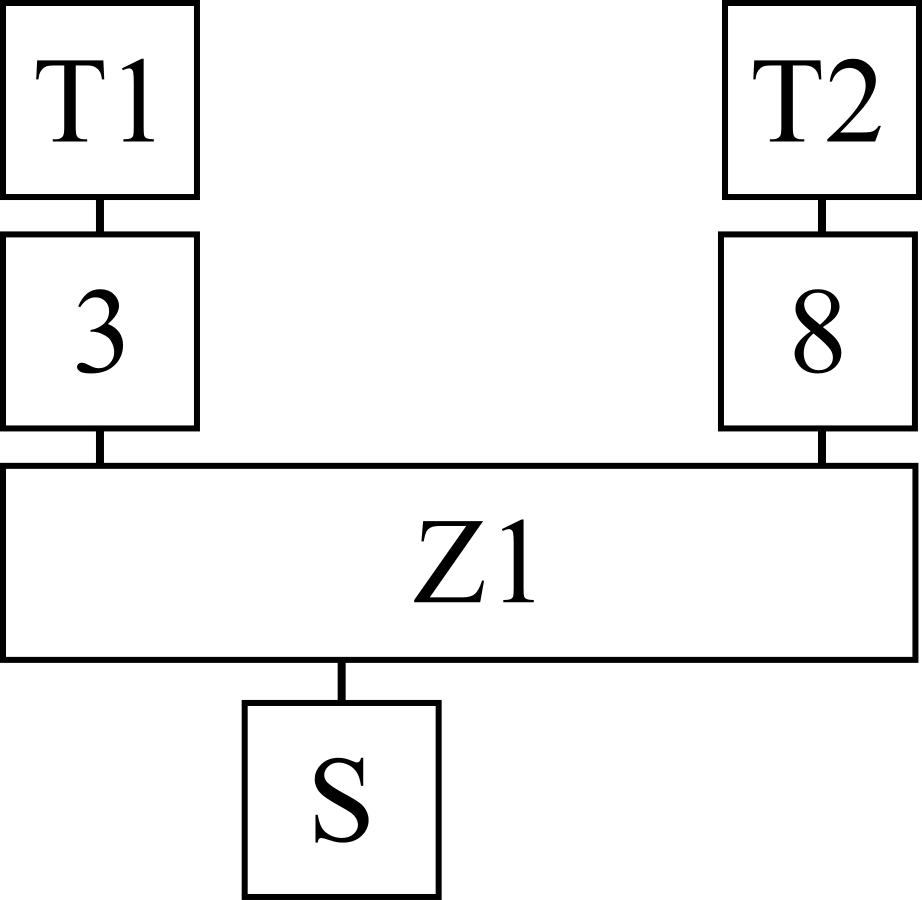
\includegraphics[scale=.15]{shadow2}
  \end{center}

  \caption{A partially observable graph with two shadow sets.}
  \label{fig:shadow2}
\end{figure}

The graph in Figure~\ref{fig:shadow2} has two disjoint shadow sets, one composed of states $2$ and $3$, the other composed of states $4$ and $5$. In using the Whale Method, the observer treats each shadow set a single state, which we will call a "whale state." We can identify the single shadow set in Figure~\ref{fig:shadow1}, composed of states $4$, $5$, $6$, and $7$. In using the Whale method, the observer treats each state in the shadow set as the same state. While the adversary may require several turns to travel among states $4$, $5$, $6$, and $7$, the adversary will act as if the has decided to remain stationary in the newly created state $W$ seen in Figure~\ref{fig:shadow3}

\begin{figure}[h!]
\begin{center}

  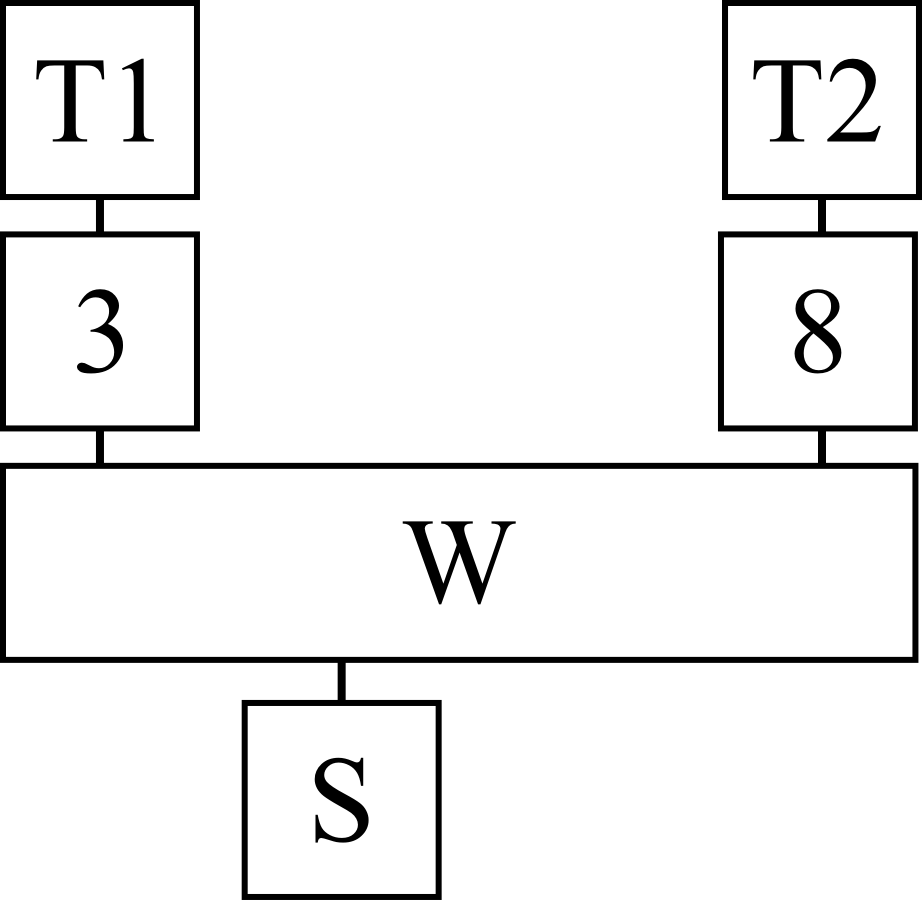
\includegraphics[scale=.15]{shadow3}
  \end{center}

  \caption{A partially observable graph with a single state in place of shadow states.}
  \label{fig:shadow3}
\end{figure}

We can add the following to the mixed integer program to accommodate for partially observable environments when using the Whale method.


\begin{equation}
V(\theta, s) \leq \sum_{i \in B} r(s, i, j, \theta)f_{i}(s) + V(\theta, j) \forall\theta\in B,\forall s \mid s\neq \theta, s\not\in H, \forall j\in\nu(s) \tag{3}
\end{equation}

\begin{equation}
V(\theta, s) \leq \sum_{i \in B} r(s, i, j, \theta)f_{w}(s) + V(\theta, j) \forall\theta\in B,\forall s \mid s\neq \theta, s\in H, \forall j\in\nu(s) \tag{3}
\end{equation}

\begin{equation}
\sum_{i} f_{i}(s) = 1\quad \forall s \tag{3}
\end{equation}

\begin{equation}
\sum_{w} f_{w}(s) = 1\quad \forall s \tag{3}
\end{equation}

\begin{equation}
f_{i}(s) \geq 0\quad \forall s,i\
\end{equation}

\begin{equation}
f_{w}(s) \geq 0\quad \forall s,w\
\end{equation}

We let $H$ denote the set of all shadow states, and $w$ denote the whale state the observer knows the adversary to be occupying. An observer action for any whale state $w$ is written as $f_{w}(s)$. These changes to the linear program require the observer to take the same action for each turn the adversary spends in a particular shadow set. The performance of the Whale method will be examined in a later section. 

\section{The Transmogrification Method}

When using the Whale method, the observer ignores some of the information available to them. The Whale method does not account for where the adversary entered a shadow set, or how long the adversary has remained hidden. The "Transmogrification Method" takes both of these pieces of information into account, by generating a fully observable environment from a partially observable environment.

\begin{figure}[h!]
\begin{center}

  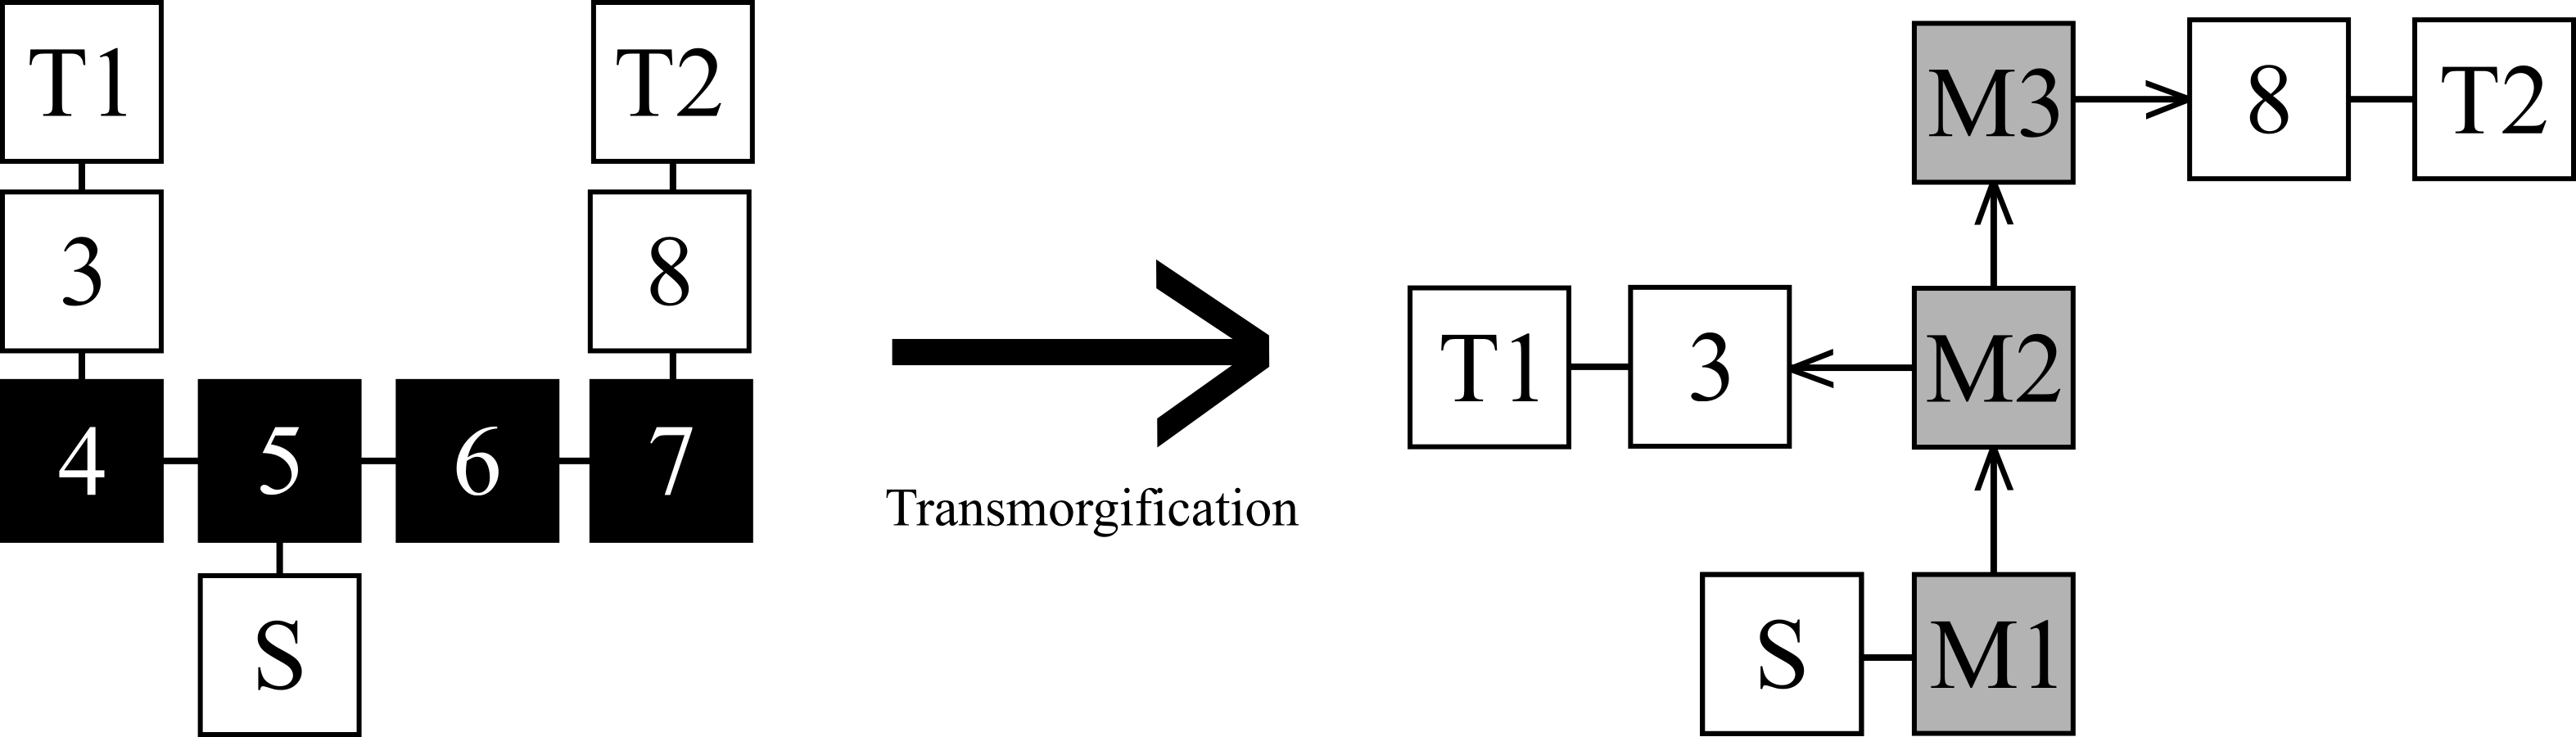
\includegraphics[scale=.15]{shadow4}
  \end{center}

  \caption{The partially observable environment from Figure~\ref{fig:shadow1} (left) transmogrified into an, fully observable graph.}
  
  \label{fig:shadow4}
\end{figure}

\nocite{Dijkstra80}
\nocite{plop03-paper}
